 \setlength{\baselineskip}{20pt}
\chapter{单帧结构感知的端到端停车位检测方法}
\label{cha:chap3}

\section{研究动机}
随着智能驾驶技术的快速发展，自动泊车系统已成为提升驾驶便利性与安全性的关键模块，而停车位检测作为自动泊车感知系统的基础，其准确性直接决定了泊车路径规划与运动控制的可靠性。

在前一章成功构建大规模停车位数据集 CRPS-D 并提出半监督训练框架 SS-PSD 的基础上，如何进一步提升停车位检测在单帧条件下的结构表达能力成为新的关键挑战。停车位本质上由多个关键点及其几何关系共同定义，具有显著的结构属性，但部分现有方法仍将停车位检测视为局部特征预测问题，依赖启发式规则对检测结果进行后处理组合，导致结构一致性难以保证，在停车位密集或局部遮挡场景下容易出现匹配错误。

从建模角度深入分析，停车位检测的核心难点不在于单个关键点的定位精度，而在于关键点之间结构关系的合理建模与约束。若结构信息未能在训练阶段得到充分利用，即便单点检测精度较高，也难以保证最终检测结果的整体结构一致性与稳定性。因此，有必要从建模范式上重新审视停车位检测问题，将结构约束显式引入模型优化过程。

当前端到端检测框架普遍面临三个主要问题：一是关键点之间的结构关系建模不充分，导致复杂拓扑下车位边界易重构错误；二是环境变化带来的样本异质性显著，如低光照、遮挡或背景干扰等情况会影响模型对局部关键点特征的准确感知；三是现有训练策略与损失函数多关注点位回归准确性，忽视点间拓扑一致性约束，无法有效引导模型学习更具结构感知能力的表示。

针对上述问题，本章提出单帧结构感知的端到端停车位检测方法，该方法以关键点表示为核心，通过在端到端训练过程中引入停车位内部结构关系约束，实现关键点定位与结构匹配的联合优化，避免对启发式后处理规则的依赖，为复杂场景下的停车位检测提供更加稳定一致的单帧建模方案。

具体而言，在检测框架设计中引入结构建模增强机制以提升车位重构稳定性，同时从损失函数与数据增强角度出发，设计结构感知的训练优化策略，以更好适应实际场景中结构不完整、样本稀疏与干扰显著的问题。综合实验验证表明，该方法在多种典型复杂环境下均具备良好的检测精度与稳定性，展现出较强的实际应用潜力。


\section{方法介绍}

本节详细介绍单帧结构感知的端到端停车位检测方法，该方法旨在解决复杂环境下停车位的稀疏关键点检测与结构匹配问题，通过引入结构感知的数据增强策略、特征插值机制与稀配聚焦损失函数，有效提升模型在低标注密度下的鲁棒性与泛化能力。

\subsection{模型框架}


\begin{figure}[!h]
\centering
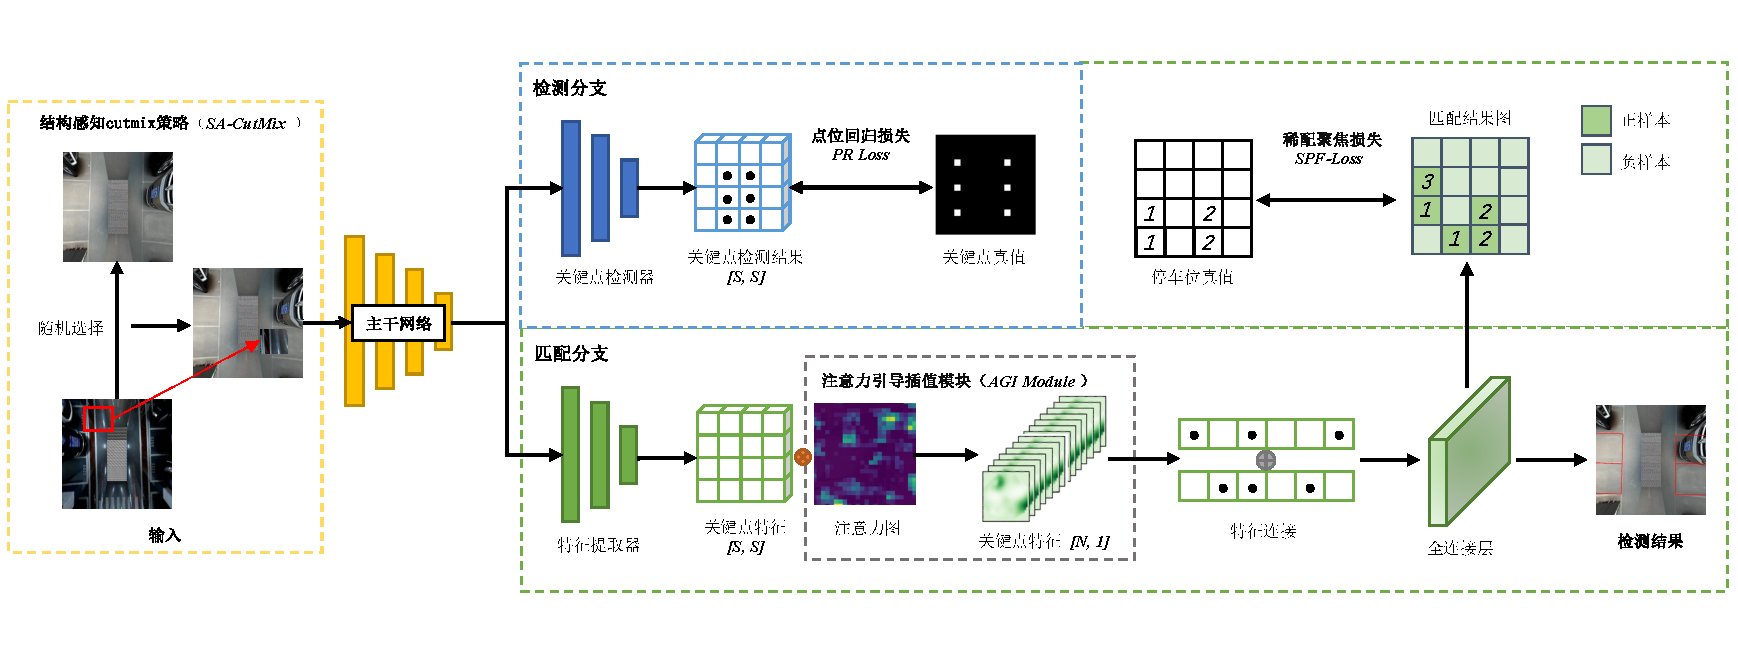
\includegraphics[width=1\textwidth]{figures/chp3/pipline_2.pdf}
\caption{单帧结构感知的端到端停车位检测框架示意图 \\Fig~\ref{fig_pip2}~Overview of the single-frame structure-aware end-to-end parking slot detection framework}
\label{fig_pip2}
\end{figure}

如图 \ref{fig_pip2} 所示，所提出的方法采用双分支架构，包含关键点检测分支与匹配分支。关键点检测分支负责提取图像中的停车位关键点位置，匹配分支则基于检测结果构建候选点对，进行结构匹配判断并生成最终停车位位置。输入图像首先经过主干特征提取网络处理，随后分流至两个分支执行各自任务。

为提升模型的结构感知能力与鲁棒性，该框架引入三项核心设计：

\textbf{结构感知 CutMix 策略（Structure-Aware CutMix，SA-CutMix）}：通过在背景区域进行智能裁剪替换，增强背景多样性的同时保持关键点结构完整性，提高模型对非结构区域的鲁棒性。

\textbf{注意力引导插值模块（Attention-Guided Interpolation，AGI Module）}：利用注意力机制引导特征插值，提升特征对关键结构位置的敏感性与表示能力。

\textbf{稀配聚焦损失（Sparse Pairwise Focal Loss，SPF-Loss）}：针对停车位关键点稀疏分布的特点，设计聚焦损失函数，缓解样本稀疏带来的训练不稳定问题。

下面将依次对这三个关键组件进行详细阐述。

\subsection{结构感知CutMix策略}
在关键点检测任务中，数据分布不均衡与场景复杂性会对模型泛化能力造成挑战，数据增强策略因此成为训练过程的关键组成部分。CutMix\cite{yun2019cutmix} 是一种经典的增强方法，通过在不同图像间随机裁剪并粘贴区域，线性混合标签信息，显著提升模型鲁棒性与抗过拟合能力。然而，原始 CutMix 未考虑空间结构语义，直接随机裁剪替换区域，在结构化感知任务中可能引发严重问题。

\begin{figure}[!h]
\centering
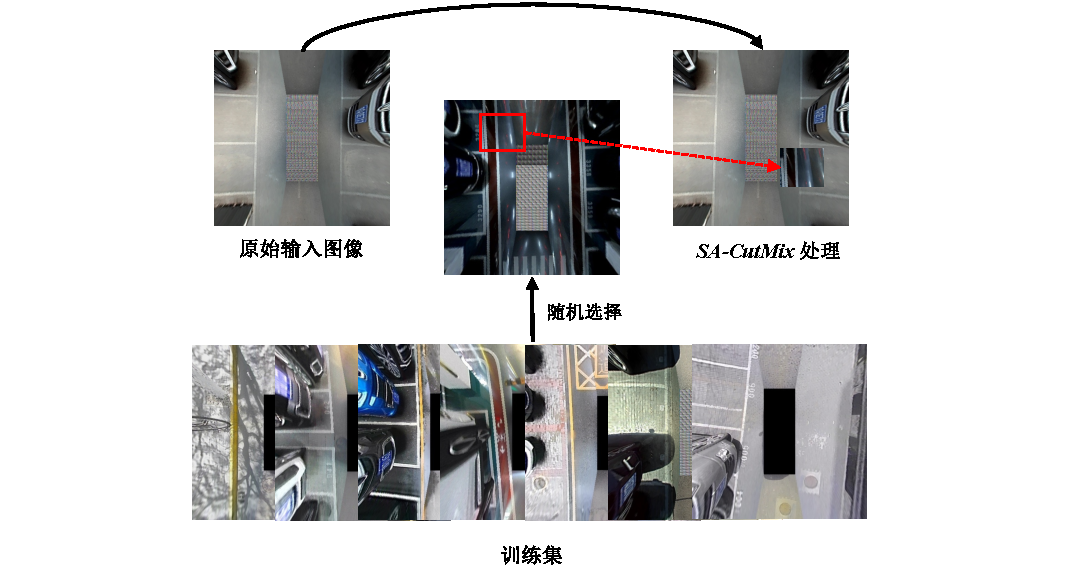
\includegraphics[width=1\textwidth]{figures/chp3/sa.pdf}
\caption{结构感知 CutMix 策略示意图 \\Fig~\ref{fig_cutmix}~Illustration of the Structure-Aware CutMix strategy}
\label{fig_cutmix}
\end{figure}

以停车位关键点检测为例，关键点稀疏且结构性强，具有明确的几何构型与位置分布规律。原始 CutMix 可能无意中裁剪关键点所在区域，打断空间几何关系，使模型难以学习结构先验，影响定位精度与稳定性。
为克服上述局限，本文提出结构感知 CutMix 策略（SA-CutMix），旨在保留结构语义信息的同时引入多样化背景扰动，兼顾数据多样性与几何结构稳定性。SA-CutMix 的核心理念是仅在背景区域进行替换操作，避免破坏关键点区域的空间结构特征。图\ref{fig_cutmix}展示了 SA-CutMix 的整体流程。

具体而言，对于每张训练图像，SA-CutMix 首先提取所有标注关键点的坐标信息，然后随机采样矩形裁剪区域作为候选替换区域。对每个候选区域，检查是否与关键点区域重叠，若有交集则视为包含结构语义信息，直接舍弃。仅当候选区域完全处于背景区域（不包含任何关键点）时，才从另一张随机选取的图像中提取相同大小的图像块进行粘贴替换。为确保算法效率，设置最大尝试次数，若未能采样到合法区域则跳过本轮增强。

该策略可概括为如下伪代码流程：

\begin{algorithm}[htbp]
\caption{结构感知 CutMix 数据增强（SA-CutMix）}
\label{alg:sacutmix}
\begin{algorithmic}[1]
\Require 当前样本图像 $I_1$，关键点坐标 $M_1$，数据集 $\mathcal{D}$
\Ensure 增强后的图像 $I_{\text{mix}}$
\If{$|\mathcal{D}| < 2$}
    \State \Return $(I_1, M_1)$ \Comment{样本不足，跳过 CutMix}
\EndIf
\Repeat
    \State 从 $\mathcal{D}$ 中随机选择 $(I_2, M_2)$，且 $I_2 \neq I_1$
    \State 在图像中随机生成矩形区域 $(x, y, w, h)$
\Until{该区域不包含 $M_1$ 中的关键点}
\State 用 $I_2$ 中对应区域替换 $I_1$ 中 $(x:x+w, y:y+h)$ 区域
\State 得到增强图像 $I_{\text{mix}}$
\State \Return $(I_{\text{mix}}, M_1)$
\end{algorithmic}
\end{algorithm}
 
SA-CutMix 从结构保持与信息干扰两个角度出发：一方面保留关键点对应的几何结构区域，使模型持续学习结构先验；另一方面引入其他图像的背景扰动，如不同地面材质、纹理变化、光照条件或遮挡物体，有效扩展模型对环境变化的感知能力。
与原始 CutMix 相比，SA-CutMix 更适用于关键点稀疏、结构约束强的任务场景。在停车位检测中，关键点数量有限且排列规律显著，任何对结构区域的破坏都可能导致空间推理能力下降。SA-CutMix 避免了这种破坏，在结构稳定的前提下引入背景扰动，增强模型对边缘遮挡、复杂纹理与极端光照等复杂场景的适应能力。

实验评估表明，SA-CutMix 的引入对模型性能具有显著提升作用。在多个遮挡与干扰条件下，模型的定位准确性与边界鲁棒性均有提升，验证了该策略在结构感知数据增强中的有效性与普适性。

\subsection{注意力引导插值模块}
在停车位关键点检测与匹配任务中，特征的精细建模对于稀疏关键点的准确定位与结构关系的稳定建模至关重要。传统描述符提取方法多采用直接在特征图上进行双线性插值采样的方式，尽管具备一定的连续性和可微性，但对所有空间位置一视同仁，未能显式区分结构区域与背景区域的重要性差异。在复杂场景中，如存在遮挡、强光、阴影或纹理混杂等干扰时，这种等权采样机制往往会削弱关键结构区域的表达能力，导致描述符判别性不足，影响后续的匹配与回归性能。

为此，本文提出注意力引导的特征插值模块（AGI Module），通过引入轻量注意力机制提升特征在结构区域的表达能力，增强描述符对结构关系的建模效果。具体地，设输入特征图为 $F\in R^{B\times C\times H\times W}$，其中 $B$ 为 batch 大小，$C$ 为通道数，$H,W$ 为特征图尺寸。首先通过 $1\times1$ 卷积操作提取通道注意力响应，生成单通道注意力图 $A\in R^{B\times1\times H\times W}$，并使用 Sigmoid 激活函数将其归一化至区间 $\left[0,1\right]$，以获得每个空间位置的显著性估计：
\begin{equation}
    A=\sigma\left({\mathrm{Conv}}_{1\times1}\left(F\right)\right)
\end{equation}

该注意力图反映当前图像中结构区域的重要性分布，可用于强调具有结构语义的显著区域并抑制冗余或噪声背景。随后，原始特征图与注意力图逐元素相乘，得到加权特征图 $F\prime=F\odot A$，该操作在保留空间连续性的同时增强了结构敏感区域的响应，有助于提升后续插值描述符的判别性。

在加权特征图 $F\prime$ 上，继续采用双线性插值对关键点位置进行特征采样。考虑到关键点位置以归一化坐标 $\left[-1,1\right]$ 表示，具体采样过程通过 PyTorch 的 $F.grid\_sample$ 函数实现，并将结果沿空间维度展平，得到结构感知描述符 $D\in R^{B\times C\times N}$，其中 N 表示每张图像中的关键点数量。由于注意力机制已对特征图进行重加权，该描述符在稀疏标注条件下表现出更强的稳定性与区分能力。整个过程如图\ref{fig_agi}所示：

\begin{figure}[!h]
\centering
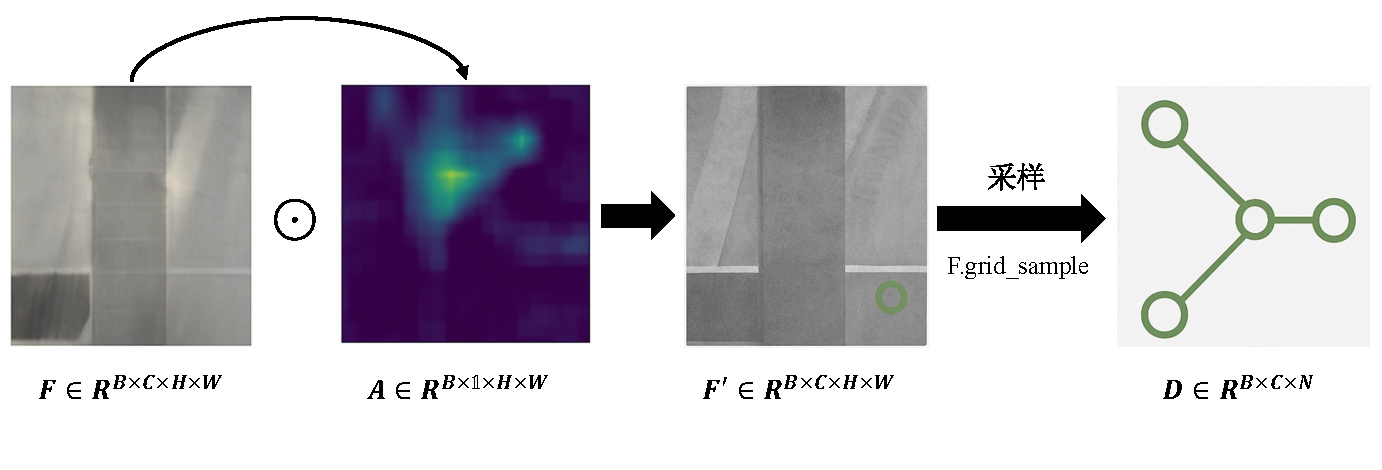
\includegraphics[width=1\textwidth]{figures/chp3/agi.pdf}
\caption{注意力引导插值模块示意图 \\Fig~\ref{fig_agi}~Illustration of the Attention-Guided Interpolation Module}
\label{fig_agi}
\end{figure}

与传统直接插值方法相比，AGI 模块通过显式建模区域重要性信息，引导描述符采样过程更加聚焦于结构显著区域，避免了背景干扰对特征表达的稀释效应。同时，AGI 模块设计简单、计算开销极小，易于集成到现有网络结构中并保持端到端训练流程。在实际停车位检测任务中，该模块在多个复杂环境下均展现出良好的泛化能力和鲁棒性，实验结果表明其对关键点检测精度和匹配稳定性均具有显著提升，进一步验证了结构引导特征建模在场景感知任务中的重要性与有效性。

\subsection{损失函数设计}
在端到端的停车位检测任务中，模型需要同时具备两项核心能力：一是精确预测图像中的停车位关键点位置，二是正确判断关键点之间是否属于同一停车位的结构关系。这两个子任务分别对应空间定位与结构理解两个方向，是最终构建完整停车位边界的必要前提。

为此，本文设计了专门的监督机制：点位回归损失（Point Regression Loss, PR-Loss）和稀配聚焦损失（Structure-aware Pairwise Focal Loss, SPF-Loss）。通过联合优化这两个损失项，模型能够在空间定位和结构关系建模两个层面上同步学习，获得更加完整和鲁棒的停车位检测能力。

（1）点位回归损失（PR-Loss）

为实现像素级的关键点定位精度，本文引入点位回归损失，用于监督模型精确预测关键点在特征图中的空间分布。该损失直接作用于从注意力增强后的特征图中回归出的置信度图及偏移信息。

本文将关键点表示为三通道张量：第一通道为关键点存在的置信度，后两通道为相对偏移 x,y。标签张量与 mask 通过以下策略构建：

a.置信度通道中，仅在真实标记点位置处置为 1；

b.偏移通道中记录该点在网格内的相对偏移；

c.mask 中标记出参与训练的位置，用于规避空区域的梯度干扰。


模型输出的点位预测结果与标签进行逐点比较，计算方式如下：
\begin{equation}
    \mathcal{L}_\mathrm{\mathrm{PR}}=\frac{1}{N_{\mathrm{mask}}}\left.\ |\left(\hat{T}-T\right)\odot M\right.|_2
\end{equation}

其中，$\hat{T}, T\in R^{B\times3\times H\times W}$ 分别表示预测与标签张量，$M$ 为 mask，$\odot$ 表示逐元素乘法，$N_{\mathrm{mask}}$ 为 mask 中非零位置的数量。损失计算时分别对置信度与偏移误差加权平均。该设计不仅提升了关键点位置的回归精度，同时使模型在关注结构区域时具备更强的几何稳定性，进一步增强了特征匹配的定位一致性。

（2）稀配聚焦损失（Structure-aware Pairwise Focal Loss, SPF-Loss）

关键点匹配任务本质上可视为一个二分类问题，即判断任意两个候选关键点是否构成真实匹配对。传统方法常采用 Binary Cross Entropy（BCE）损失，但在“结构模糊区域”中，例如存在遮挡、模糊或车位密集的情况下，模型往往难以聚焦于困难样本，容易出现误匹配。为此，本文提出稀配聚焦损失（SPF-Loss），引入焦点机制增强对难匹配样本的关注，同时结合结构约束以提升对稀疏边对的判别能力，从而提高整体匹配精度与鲁棒性。

具体而言，首先构建大小为 $N \times N$ 的匹配预测矩阵 $P=\{p_{ij}\}$，其中每个元素表示图像对中第 i 个关键点与第 j 个关键点的匹配置信度。同时构建标签矩阵 $Y=\{y_{ij}\}$，其中 $y_{ij}=1$ 表示正匹配对，$y_{ij}=2$ 表示负匹配对，$y_{ij}=0$ 表示无效对。此外，定义有效掩码 $M_{ij}=\mathbb{1}\left(y_{ij}>0\right)$，仅对有效匹配对（正负样本）计算损失，以排除对模型无意义的区域干扰。

本文采用 Focal Loss\cite{lin2017focal} 的形式，将传统 BCE 扩展为：
\begin{equation}
    \mathcal{L}_\mathrm{SPF}=-\frac{1}{N_{\mathrm{valid}}}\sum_{i,j} M_{ij}\cdot\left[\alpha\left(1-p_{ij}\right)^\gamma y_{ij}^\prime\log{\left(p_{ij}+\varepsilon\right)}+\alpha p_{ij}^\gamma\left(1-y_{ij}^\prime\right)\log{\left(1-p_{ij}+\varepsilon\right)}\right]
\end{equation}

其中，$p_{ij}$ 表示模型预测的匹配概率，$\alpha$ 为类别权重调节因子，$\gamma$ 控制聚焦程度，$\varepsilon$ 是为防止数值不稳定引入的微小常数，$N_{\mathrm{valid}}$ 为所有有效点对数量。由于 Focal Loss 是专为二分类任务设计的，其要求标签为二值形式（正样本为 1，负样本为 0），因此构造二值化目标标签：
\begin{equation}
    y_{ij}\prime=\mathbb{1}\left(y_{ij}=1\right)
\end{equation}

即当 $y_{ij}=1$ 时，$y_{ij}\prime = 1$；否则为 0。该设计不仅解决了原始多标签匹配信息与 Focal Loss 结构不兼容的问题，同时避免了无效区域带来的梯度干扰，使得模型能更加关注边界模糊、结构遮挡、复杂形状干扰等困难匹配场景，训练过程中自动对高难度匹配对赋予更大梯度，从而显著提升结构推理能力。

（3）总损失函数

上述两种损失在训练过程中被共同优化，整体损失函数形式为：
\begin{equation}
    \mathcal{L}_\mathrm{total}=\lambda_1\cdot\mathcal{L}_\mathrm{PR}+\lambda_2\cdot\mathcal{L}_\mathrm{SPF}
\end{equation}

其中，$\lambda_1、\lambda_2$为损失项的加权系数，用于平衡结构判别与点位回归的相对重要性。实验表明，该损失设计能够有效提升模型在复杂环境下的匹配鲁棒性与几何一致性，尤其在面对结构遮挡、视角变化或多目标干扰等挑战性场景时，性能提升显著。本文选取在验证集上综合性能最优的一组权重参数，并在所有实验中保持一致。最终，点位回归损失与结构感知匹配损失的权重分别设置为 $\lambda_1 = 10，\lambda_2 = 1$。

\section{实验结果及分析}
本章所有实验均在同一硬件平台上进行，具体包括一块Nvidia 2080Ti GPU（12GB显存）和一台配备Intel(R) Xeon(R) E5-2680 v4 @ 2.40GHz CPU的服务器环境。模型训练使用PyTorch框架实现。

\subsection{对比实验}
（1）公开数据集 ps2.0

为验证所提方法的有效性，本文首先在公开数据集 ps2.0 上进行了充分的对比实验。ps2.0 数据集作为当前视角停车位检测任务中最具代表性和广泛使用的基准数据集之一，涵盖了多种典型的室内外停车场景，被众多主流方法用于性能评估。该数据集中，已有方法的检测精度普遍较高，查准率（Precision）和查全率（Recall）均达到 99\%左右，整体性能趋于饱和。

\begin{table}[!ht]
\centering
\setlength{\tabcolsep}{5mm}
\caption{不同方法在 ps2.0 数据集上的检测性能对比 \\
Table~\ref{tab_2ps2}~Comparison of detection performance of different methods on ps2.0 dataset}
\begin{tabular}{lccccc}
\toprule
    方法 &  Precision & Recall &  AP\\
\midrule
       DeepPS\cite{zhang2018vision}  &  98.99\% & 99.13\% & / \\
       DMPR-PS\cite{huang2019dmpr} &  99.42\% & 99.37\% & / \\
       VPS\cite{li2020vacant}  &  99.63\% & 99.10\% & / \\
       GCN\cite{min2021attentional}  &  99.56\% & 99.42\% & /\\
       SCCN \cite{zheng2022center}  &  99.35\% & 99.17\% & / \\
       Bui et al.\cite{bui2023one} &   99.63\% & 99.63\% & / \\
       SAM-PS\cite{zhai2024sam} &  94.29\% & 81.35\% & / \\
       BEV-PolyNet\cite{duan2025bev}  &  99.82\% & 99.65\% & / \\
       \textbf{Ours} &   \textbf{99.37\%} & \textbf{99.47\%} & \textbf{99.47\%}\\
\bottomrule
\end{tabular}
\label{tab_2ps2}
\end{table}

如表\ref{tab_2ps2}所示，本文方法在 ps2.0 数据集上的查准率为 99.37\%，查全率为 99.47\%，与现有先进方法保持在同一水平，充分验证了所提出方法在标准场景下的适应性和准确性。值得注意的是，本文方法是唯一在该数据集上提供平均精度（AP）指标的方法，达到了 99.47\%，进一步印证了模型在检测精度与鲁棒性方面的兼顾能力。

然而，ps2.0 数据集中场景较为规整，泊车线条清晰、遮挡情况较少，难以覆盖真实自动泊车场景中可能遇到的复杂情况，如遮挡严重、停车位密集、斜向车位增多等。因此，仅在该数据集上取得良好性能并不足以全面评估模型在真实环境中的实际应用潜力。为此，本文进一步引入具有更高挑战性和复杂度的私有数据集 CRPS-D，并在该数据集上进行了更具代表性的对比实验，以验证所提方法在复杂场景下的泛化能力与鲁棒性。

（2）新数据集CRPS-D

在进一步的实验中，本文在上一章构建的CRPS-D数据集上对所提方法进行了深入评估。鉴于目前大多数端到端停车位检测方法尚未公开训练代码或预训练模型，难以在统一平台和设置下在CRPS-D上实现全面复现与公平对比。在已公开的方法中，仅有GCN\cite{min2021attentional}提供了完整的训练框架，并支持多种主干网络（ResNet18、ResNet50、Darknet、VGG16），具备良好的可复现性与扩展性。因此，本文选取GCN作为对比基线，在保持数据集、损失函数、训练策略和超参数一致的前提下，基于相同的四种主干网络在CRPS-D数据集上进行了复现训练，并与本文方法进行了系统的对比实验。

\begin{table}[!h]
\centering
\setlength{\tabcolsep}{4mm}
\caption{本文方法与 GCN\cite{min2021attentional} 在 CRPS-D 数据集上的检测性能对比 \\
Table~\ref{tab_2crps}~Comparison between the proposed method and GCN\cite{min2021attentional} on CRPS-D dataset}
    \begin{tabular}{lccccc}
        \toprule
         方法 & 主干网络 & Precision & Recall & AP & AP提升 \\
        \midrule
            GCN$^{*}$  & \multirow{2}{*}{Resnet18} & 91.38\% & 82.04\% & 78.01\%  & \multirow{2}{*}{4.37\%}\\
             本文方法  &  & 91.56\%	& 84.54\%	& 82.38\%  & \\

        \midrule
             GCN$^{*}$  & \multirow{2}{*}{Resnet50} & 90.91\%	& 83.22\%	& 78.63\%  & \multirow{2}{*}{3.47\%}\\
             本文方法  &  & 91.11\% &	84.89\%	& 82.10\%	  & \\
        \midrule
              GCN$^{*}$  & \multirow{2}{*}{Darknet} & 91.38\%	& 83.27\%	& 79.01\%  & \multirow{2}{*}{3.92\%}\\
             本文方法  &  & 91.39\% &	85.00\%	& 82.93\%	  & \\
        \midrule
              GCN$^{*}$  & \multirow{2}{*}{Vgg16} & 92.43\%	& 82.75\%	& 79.02\%  & \multirow{2}{*}{4.56\%}\\
             本文方法  &  & 92.21\%	& 85.54\%	& 83.58\%  & \\
        \bottomrule
    \end{tabular}
    \label{tab_2crps}
\end{table}

实验结果如表\ref{tab_2crps}所示，本文方法在四种主干网络下均实现了对 GCN 方法的全面超越，特别是在关键指标 AP 上取得了显著提升。其中，基于 VGG16 的配置下，本文方法的 AP 达到 83.58\%，相较 GCN 的 79.02\%，提升了 4.56 个百分点，体现出在较深网络结构下的更强表达能力。在 ResNet18、ResNet50 和 Darknet 主干下，AP 也分别提升了 4.37\%、3.47\% 和 3.92\%，平均提升约 4.08\%。该结果表明，本文方法在不同主干结构下均具备良好的兼容性和稳定性，能够有效挖掘停车位的结构信息，提升检测性能。

此外，从表格数据可以看出，在查准率保持相对稳定的同时，本文方法在查全率方面有明显增长。例如，在 VGG16 主干下，查全率从 82.75\% 提升至 85.54\%，增长了 2.79 个百分点；在 ResNet18 主干下，查全率从 82.04\% 提升至 84.54\%，增长了 2.50 个百分点。这表明本文方法在面对复杂、密集、非规则停车位分布场景时，具备更强的目标捕获能力，同时保持了较高的检测精度。这种能力的提升对于实际自动泊车系统中的可靠检测至关重要，特别是在遮挡、光照变化、车位倾斜和空间紧凑等真实条件下。

\subsection{消融实验}

为进一步验证本文所提出各模块与设计的有效性，本文在 CRPS-D 数据集上进行了消融实验。实验采用ResNet18作为主干网络，依次引入关键设计组件，包括 AGI模块、 SPF-loss 以及 SA-CutMix 数据增强策略，并在保持其他设置不变的前提下，观察各组件对模型性能的影响。实验结果如表 \ref{tab_2ab} 所示。

\begin{table*}[!h]
\centering
\setlength{\tabcolsep}{4mm}
\caption{模块逐步引入对模型性能的影响 \\
Table~\ref{tab_2ab}~Impact of incremental module integration on detection performance}
\small
\begin{tabular}{ccccc}
\toprule
    Baseline(仅主干网络) & AGI Module & SPF-Loss  & SA-CutMix &  $AP_{parking-slot}$ \\
\midrule
    \checkmark  &  &  &  &  77.76\% \\
     \checkmark & \checkmark &  &  &  78.94\% \\
     \checkmark & \checkmark & \checkmark &  &  79.45\% \\
     \checkmark & \checkmark & \checkmark & \checkmark  & \textbf{82.38\%} \\
\bottomrule
\end{tabular}
\label{tab_2ab}
\end{table*}

从实验结果可以看出，所提出的每个模块均对最终性能有积极贡献，且呈现出累加效应。首先，在基准模型中引入AGI模块后，AP从 77.76\%提升至 78.94\%，提升了 1.18 个百分点，表明该模块在捕捉车位关键点间的几何关系方面具备良好的建模能力。进一步加入 SPF-Loss 后，AP 提升至 79.45\%，显示结构感知损失函数能有效增强模型对关键点间结构匹配的关注，从而提高整体检测精度。最后，结合 SA-CutMix 数据增强策略后，AP 显著提升至 82.38\%，进一步提升了模型的泛化能力和鲁棒性。

综上所述，本文各关键设计均能在不同程度上提升模型性能，且组合使用时效果最优，验证了本文提出方法在结构建模、损失设计和数据增强等方面的有效性和互补性。各模块协同工作，共同提升了模型在复杂场景下的检测性能。

\subsection{可视化结果}
为进一步验证本文方法在实际应用中的泛化能力与鲁棒性，本文从 CRPS-D 数据集中选取了十种具有代表性的复杂场景进行可视化展示，如图 \ref{fig_res2} 所示。所选场景涵盖了多种真实环境下的典型干扰因素，包括光照条件多变（如室内弱光、强光、夜间和强阴影）、恶劣天气（如雨天）、结构复杂性（如斜置车位和受损车位），以及车位分布密集或地面存在反光等情形。这些场景充分模拟了实际停车环境中常见的挑战因素，对模型的感知能力和鲁棒性提出了更高要求。

\begin{figure}[!h]
\centering
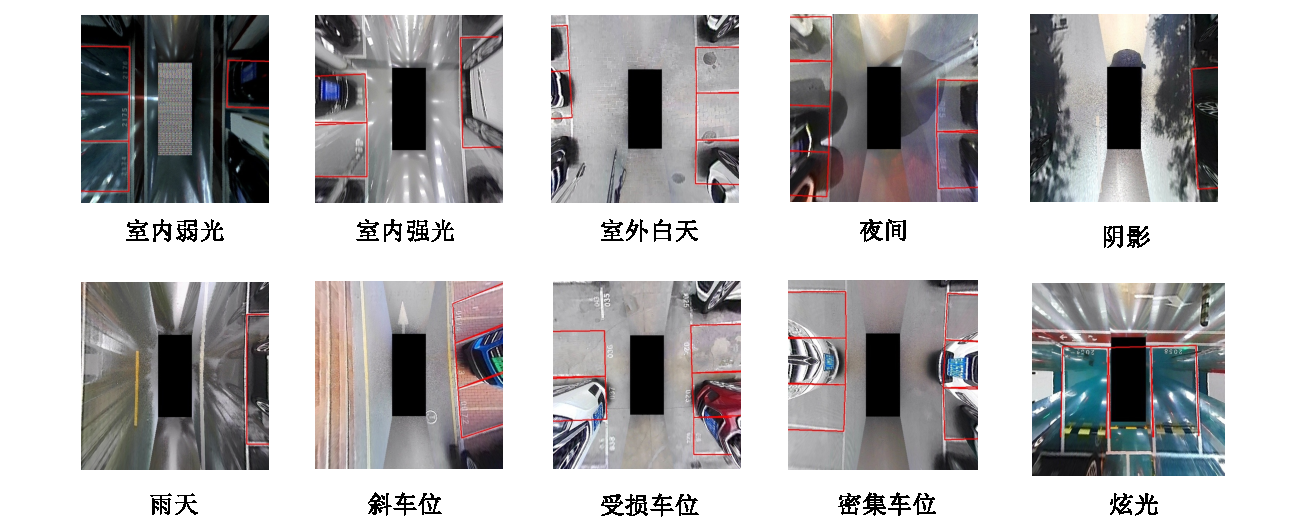
\includegraphics[width=1\textwidth]{figures/chp3/result_2.pdf}
\caption{不同场景下的可视化停车位检测结果 \\Fig~\ref{fig_res2}~Visualization results of parking slot detection under diverse scenarios}
\label{fig_res2}
\end{figure}

从图 \ref{fig_res2} 结果可以看出，本文方法在各类复杂条件下均能准确检测车位关键点，并有效构建出完整的车位结构。即使在光照不足、强反光或雨天等视觉干扰较强的场景中，检测结果仍然清晰、边界准确，未出现明显误检或漏检，展示了良好的环境适应性和稳定性。同时，在车位密集和斜置等边界难以区分的复杂场景中，方法仍表现出较高的判别能力，进一步验证了其在多样化泊车环境下的应用潜力。这些可视化结果与定量实验数据相互印证，充分展示了本文方法的有效性和鲁棒性。

\section{本章小结}

本章针对单帧条件下停车位检测中结构表达能力不足的问题，提出了一种单帧结构感知的端到端停车位检测方法，实现了关键点定位与结构匹配的联合优化。

该方法设计了双分支检测框架，通过关键点检测分支与匹配分支的协同工作，在无需额外后处理的情况下自动构建车位结构，有效融合了车位拓扑先验信息。同时，提出了三项核心技术：结构感知CutMix策略（SA-CutMix）在保持结构完整性的同时增强模型泛化能力；注意力引导插值模块（AGI Module）提升特征对结构区域的敏感性；稀配聚焦损失（SPF-Loss）增强模型对困难样本的判别能力。

实验验证表明，该方法在ps2.0和CRPS-D数据集上均取得了优异性能，在 CRPS-D 数据集上相比基线方法平均提升 AP 约 4.08\%，尤其在复杂场景下表现出更强的鲁棒性。消融实验进一步验证了各模块的有效性，其中 SA-CutMix 带来约 2.93\% 的 AP 提升，AGI模块带来约 1.18\% 的AP提升，SPF-Loss 带来约 0.51\% 的 AP 提升。

本章方法通过显式引入结构约束，有效提升了停车位检测在遮挡、密集与非标准停车形式下的稳定性与一致性，为后续引入时序信息提供了可靠的单帧结构基础。